\section{3D System Simulation}\label{sec:3d_sim}

\paragraph{}The 2D simulation in the former section serves its purpose as a simple case scenario of the problem. Whereas most of the calculations will be approached in a different way, it follows the same principle (******).
In this case, the frame will not be a simple cartesian plane, but instead we will consider the WGS84 Geodetic Standard (Section \ref{sec:geodetic}).


\paragraph{} Figure \ref{fig:diagram3D} shows the block diagram used in MATLAB Simulink in order to run this simulation. It is mainly based in the following steps:
\begin{enumerate}
\item{Read Ground Station and Drone GPS position}
\item{Calculate optimal angles (reference), error signal and other parameters. This requires from frames transformation and other functions, and it is performed inside the MATLAB function block, which will be explained later on.}
\item{Input the error signal into the controller.}
\item{Limit the output signal from the controller by the use of the saturation box.}
\item{Input output signal into Servo-motor model box. This model can be seen in Figure \ref{fig:servomotor3D}, whose parameters have been explain in Chapter \ref{sec:servo_model}.}
\item{Feedback the output angle into the MATLAB function block, repeating again from step 2.}
\end{enumerate}

\begin{figure}[h]
	\centering
	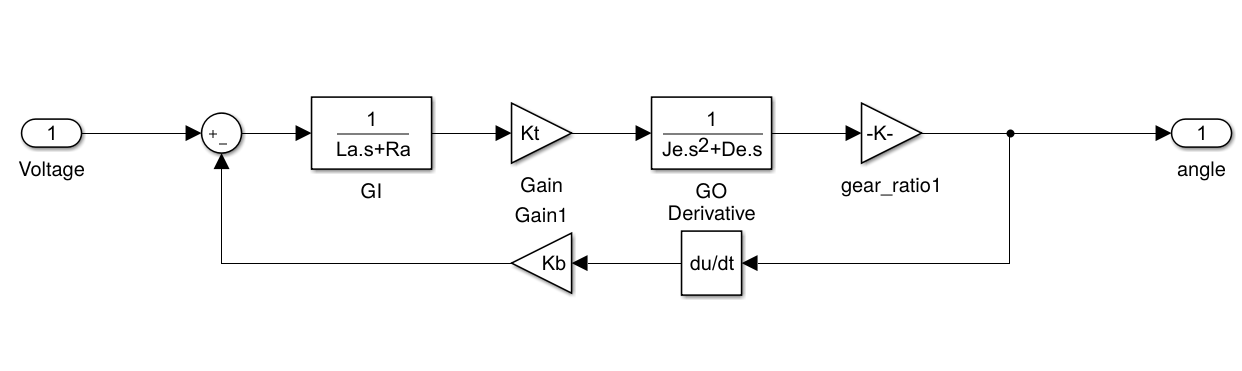
\includegraphics[width=1.1\textwidth]{figures/servomotor_3D.png}
	\caption{Servo-motor Block Diagram}
   	\label{fig:servomotor3D}
\end{figure}

\begin{sidewaysfigure}
	\centering
	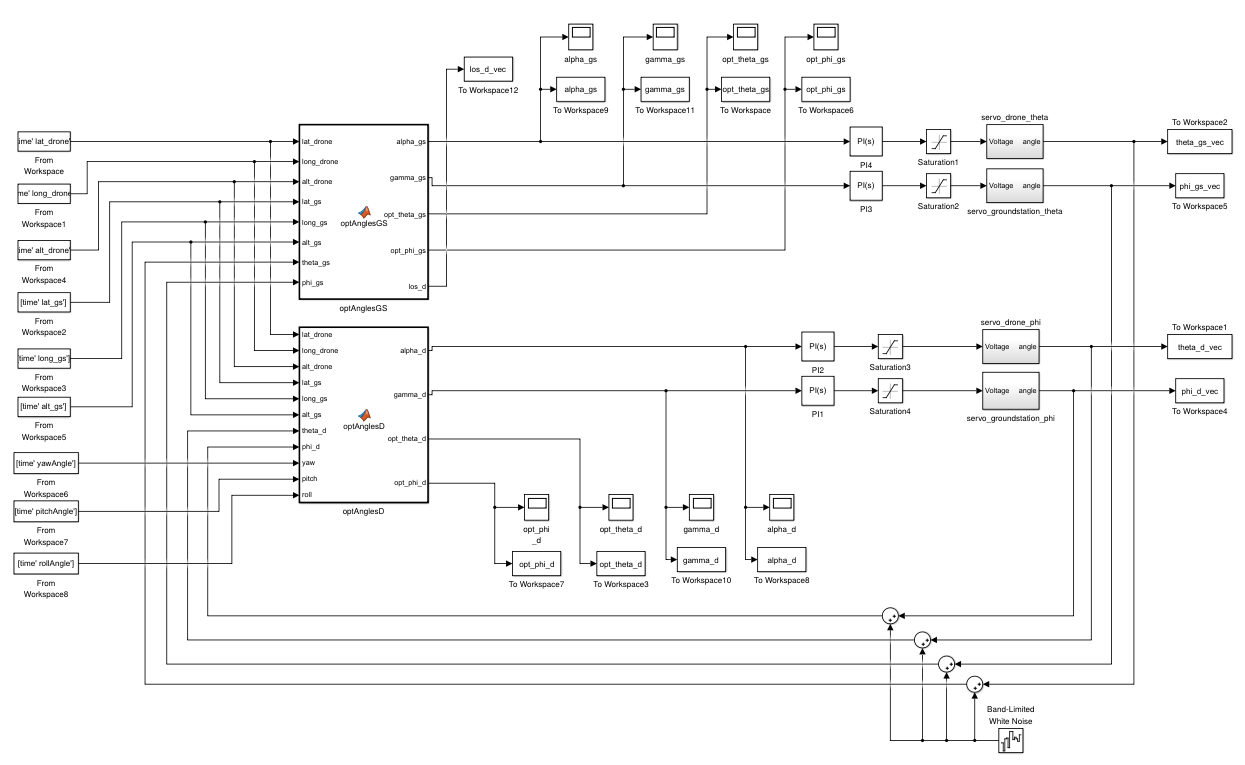
\includegraphics[width=1.1\textwidth,height=1.1\textheight,keepaspectratio]{figures/diagram_3D.png}
	\caption{Block Diagram for 3D Simulation}
   	\label{fig:diagram3D}
\end{sidewaysfigure}

Note 

\begin{figure}[h]
	\centering
	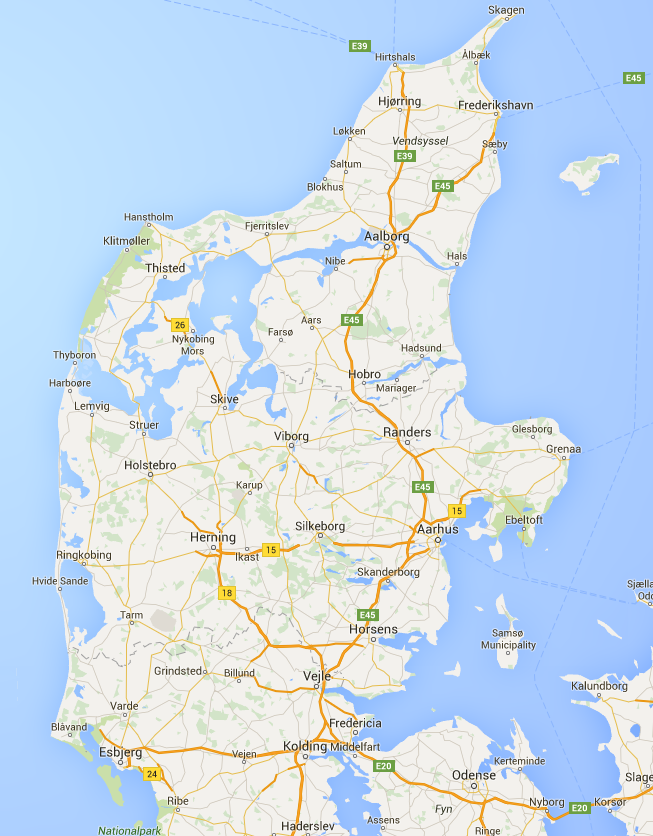
\includegraphics[width=0.5\textwidth]{figures/denmark.png}
	\caption{Denmark}
   	\label{fig:denmark}
\end{figure}

